\documentclass[11pt,a4paper]{article}

% ============================================================================
% PACKAGES
% ============================================================================
\usepackage[utf8]{inputenc}
\usepackage[T1]{fontenc}
\usepackage{lmodern}
\usepackage[margin=2.5cm]{geometry}
\usepackage{amsmath,amssymb,amsfonts,amsthm}
\usepackage{mathtools}
\usepackage{bm}
\usepackage{siunitx}
\usepackage{booktabs}
\usepackage{multirow}
\usepackage{array}
\usepackage{graphicx}
\usepackage{float}
\usepackage{caption}
\usepackage{subcaption}
\usepackage{tikz}
\usepackage{pgfplots}
\pgfplotsset{compat=1.18}
\usetikzlibrary{arrows.meta,positioning,patterns,calc,decorations.pathmorphing}
\usepackage[colorlinks=true,linkcolor=blue!70!black,citecolor=blue!70!black,urlcolor=blue!70!black]{hyperref}
\usepackage{authblk}

% Setup siunitx
\sisetup{
    separate-uncertainty = true,
    multi-part-units = single,
    per-mode = symbol
}

% ============================================================================
% TITLE & AUTHORS
% ============================================================================
\title{\textbf{A Segmented-Column Gamma-Spectrometric Method for Characterizing $^{222}\text{Rn}$ Diffusion, Adsorption Retardation, and Outlet Leakage in Activated Carbon}}

\author[1]{Hristo \textit{et al.}}
\affil[1]{Department of Nuclear Engineering / Dosimetry and Radiation Protection Laboratory}
\date{November 2026}

\begin{document}

\maketitle

% ============================================================================
% ABSTRACT
% ============================================================================
\begin{abstract}
\noindent
Activated carbon beds are widely utilized for radon ($^{222}\text{Rn}$) mitigation, delay lines, and activity concentration metrology. Accurate characterization of the effective diffusion coefficient ($D_e$), diffusion attenuation length ($L_d$), and adsorption partition coefficient ($K_a$) is essential for predicting breakthrough behavior. In this work, we present a non-destructive experimental and theoretical method for reconstructing the steady-state one-dimensional spatial profile of $^{222}\text{Rn}$ across a segmented adsorber column consisting of $N=9$ sequential activated carbon cartridges loaded via a radon emanator. Following attainment of steady-state transport and secular equilibrium between $^{222}\text{Rn}$ and its short-lived gamma-emitting progeny ($^{214}\text{Pb}$ at \SI{352}{keV} and $^{214}\text{Bi}$ at \SI{609}{keV}), the cartridges were measured sequentially in reverse order by high-resolution gamma-ray spectrometry. We derive the complete analytical solutions to the 1D diffusion-decay-adsorption equation under ideal open-end (Dirichlet), closed-end (Neumann), and leaking-end (Robin / dual-porosity bypass) boundary conditions, as well as a normalized attenuation profile relative to non-decaying linear Fickian diffusion. We also prove mathematically that integrating the hyperbolic concentration profile over a finite cartridge thickness $\Delta x$ preserves the exact functional form evaluated at the cartridge midpoint. Experimental results demonstrate a strict spatial halving law across the interior cartridges ($R_i / R_{i+1} = 1.98 \pm 0.05$), yielding a dimensionless attenuation modulus of $\mu = \Delta x / L_d = 0.686 \pm 0.008\text{ cartridge}^{-1}$ ($L_d = 1.46\,\Delta x$). Furthermore, boundary deviations at the inlet ($i=1$) and outlet ($i=9$) are quantitatively explained by post-dismantling front-face desorption and unretarded inter-granular gas leakage driven by the emanator partial pressure.

\vspace{0.3cm}
\noindent\textbf{Keywords:} Radon-222; Activated carbon; Porous media diffusion; Gamma-ray spectrometry; Thiele modulus; Robin boundary condition; Adsorption retardation.
\end{abstract}

\hruler
\tableofcontents
\vspace{0.5cm}

% ============================================================================
% 1. INTRODUCTION
% ============================================================================
\section{Introduction}
The transport of the radioactive noble gas radon ($^{222}\text{Rn}$, half-life $T_{1/2} = \SI{3.8235}{d}$, decay constant $\lambda = \SI{2.0982e-6}{s^{-1}}$) through porous media is a fundamental process in environmental physics, geological engineering, and nuclear safety. In particular, granular activated carbon (GAC) exhibits an exceptionally high physical adsorption affinity for radon due to van der Waals interactions within its microporous network (pore diameters $<\SI{2}{nm}$). Consequently, activated carbon cartridges and delay beds are extensively employed both as passive/active samplers for indoor radon dosimetry and as dynamic delay columns in nuclear facilities and rare-event physics laboratories.

When $^{222}\text{Rn}$ migrates through an activated carbon bed, its macroscopic transport rate is governed by the interplay between molecular/Knudsen diffusion in the inter-granular void space, reversible adsorption-desorption kinetics on the internal carbon surfaces, and first-order radioactive decay. In a one-dimensional (1D) slab or cylindrical column geometry at steady state, this competition establishes an exponentially or hyperbolically decaying spatial concentration profile characterized by the effective diffusion attenuation length $L_d = \sqrt{D_e / \lambda}$.

Conventional methods for determining $L_d$ and the effective diffusivity $D_e$ typically rely on measuring only the inlet and outlet gas-phase radon concentrations across a monolithic column (breakthrough method). However, two-point measurements cannot resolve internal spatial inhomogeneities, entrance saturation effects, or unretarded gas-phase channeling (leakage) through macropores. 

In this paper, we present a high-precision **segmented-column method** using $N=9$ sequential activated carbon cartridges exposed to a $^{222}\text{Rn}$ emanator. By measuring the gamma-ray emission from the short-lived radon progeny ($^{214}\text{Pb}$ and $^{214}\text{Bi}$) trapped in each individual cartridge, we directly map the internal steady-state profile $C(x)$ along the entire adsorber length. We develop a rigorous mathematical framework encompassing Dirichlet, Neumann, and Robin (leaking-end) boundary conditions, introduce a normalized attenuation transformation that isolates the radioactive decay contribution from linear Fickian transport, and validate the models against experimental spectrometric data.

% ============================================================================
% 2. EXPERIMENTAL SETUP AND MEASUREMENT PROTOCOL
% ============================================================================
\section{Experimental Setup and Measurement Protocol}

\subsection{Segmented Adsorber Column and Radon Loading}
The adsorber assembly consists of $N=9$ identical cylindrical cartridges packed with granular activated carbon, arranged coaxially in series to form a continuous 1D porous column of total length $L = N\Delta x$, where $\Delta x$ is the axial thickness of a single cartridge (Fig.~\ref{fig:setup}). 

\begin{figure}[H]
\centering
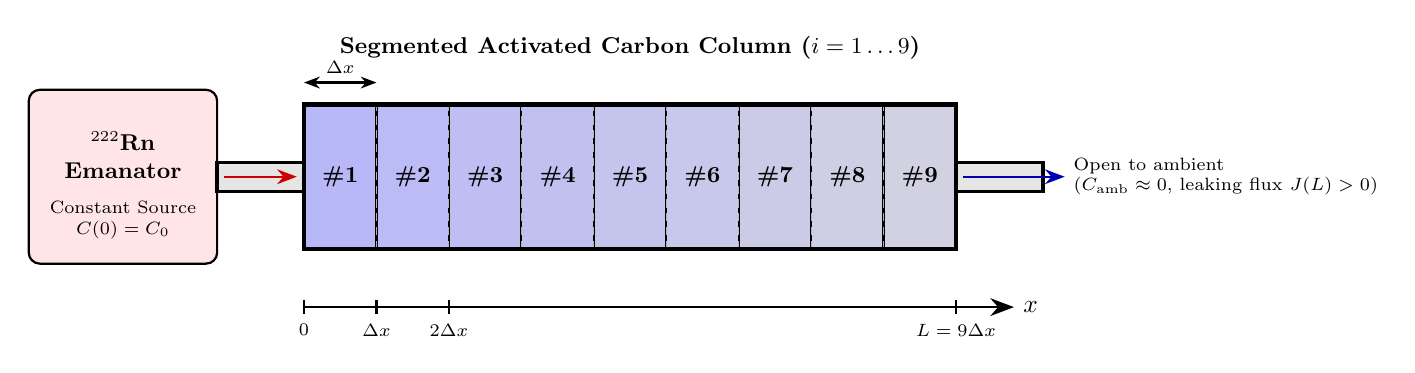
\begin{tikzpicture}[scale=0.92, every node/.style={transform shape}]
    % Radon Emanator
    \draw[thick, fill=red!10, rounded corners=4pt] (-3.8, -0.2) rectangle (-1.2, 2.2);
    \node[align=center, font=\bfseries\small] at (-2.5, 1.3) {$^{222}\text{Rn}$\\Emanator};
    \node[align=center, font=\scriptsize] at (-2.5, 0.4) {Constant Source\\$C(0) = C_0$};
    
    % Pipe from Emanator to Column
    \draw[very thick, fill=gray!20] (-1.2, 0.8) rectangle (0, 1.2);
    \draw[-{Stealth[length=2.5mm]}, thick, red!80!black] (-1.1, 1.0) -- (-0.1, 1.0);

    % 9 Cartridges
    \foreach \i in {1,...,9} {
        \pgfmathsetmacro{\xstart}{(\i-1)*1.0}
        \pgfmathsetmacro{\xend}{\i*1.0}
        \pgfmathsetmacro{\shadeval}{85 - (\i-1)*8}
        \draw[thick, fill=blue!\shadeval!gray!30] (\xstart, 0) rectangle (\xend, 2.0);
        \draw[densely dashed, gray!60] (\xstart, 0) -- (\xstart, 2.0);
        \node[font=\bfseries\small] at (\xstart+0.5, 1.0) {\#\i};
    }
    % Outer casing
    \draw[ultra thick] (0,0) rectangle (9.0, 2.0);

    % Outlet to atmosphere
    \draw[very thick, fill=gray!20] (9.0, 0.8) rectangle (10.2, 1.2);
    \draw[-{Stealth[length=2.5mm]}, thick, blue!70!black] (9.1, 1.0) -- (10.5, 1.0);
    \node[right, align=left, font=\scriptsize] at (10.5, 1.0) {Open to ambient\\($C_{\text{amb}} \approx 0$, leaking flux $J(L) > 0$)};

    % Coordinate axis
    \draw[-{Stealth[length=3mm]}, thick] (0, -0.8) -- (9.8, -0.8) node[right] {$x$};
    \foreach \x/\label in {0/$0$, 1.0/$\Delta x$, 2.0/$2\Delta x$, 9.0/$L = 9\Delta x$} {
        \draw[thick] (\x, -0.7) -- (\x, -0.9) node[below, font=\scriptsize] {\label};
    }

    % Labels above
    \draw[{Stealth[length=2mm]}-{Stealth[length=2mm]}, thick] (0, 2.3) -- (1.0, 2.3) node[midway, above, font=\scriptsize] {$\Delta x$};
    \node[above, font=\small\bfseries] at (4.5, 2.5) {Segmented Activated Carbon Column ($i = 1 \dots 9$)};
\end{tikzpicture}
\caption{Schematic representation of the experimental setup showing the $^{222}\text{Rn}$ emanator connected to the inlet of the 9-cartridge activated carbon column ($x=0$) and the open outlet at Cartridge \#9 ($x=L=9\Delta x$).}
\label{fig:setup}
\end{figure}

During the loading phase, the inlet face of Cartridge \#1 ($x = 0$) was connected directly to a calibrated $^{222}\text{Rn}$ emanator source maintaining a constant inlet concentration $C(0) = C_0$. The outlet face of Cartridge \#9 ($x = L$) was left open to the laboratory atmosphere, where the ambient radon concentration is negligible ($C_{\text{amb}} \approx 0$). 

Because the emanator imposes a finite partial pressure and chemical potential gradient of radon across the column, two transport regimes coexist within the granular bed:
\begin{enumerate}
    \item \textbf{Retarded Micropore Diffusion:} Radon molecules diffusing into the internal micropores of the carbon grains undergo strong physical adsorption, slowing their effective migration rate by several orders of magnitude and allowing radioactive decay to attenuate the concentration by a factor of $\sim 2$ per cartridge.
    \item \textbf{Unretarded Inter-Granular Leakage:} A small fraction of the gas migrates through the inter-granular macropores without strong adsorption retardation, maintaining a small but non-zero leaking flux $J(L) > 0$ at the outlet face of Cartridge \#9.
\end{enumerate}

\subsection{Gamma-Ray Spectrometry Protocol}
Once steady-state radon distribution and secular equilibrium between $^{222}\text{Rn}$ and its short-lived progeny ($^{218}\text{Po}$, $^{214}\text{Pb}$, $^{214}\text{Bi}$, and $^{214}\text{Po}$) were established, the column was disconnected and disassembled into its 9 constituent cartridges. 

To avoid detector cross-contamination and minimize dead-time losses during the initial measurements, the cartridges were measured sequentially in **reverse order**—starting from the lowest-activity outlet cartridge ($i = 9$, measured at $\text{10:16:34}$) and progressing to the highest-activity inlet cartridge ($i = 1$, measured at $\text{12:25:47}$). Each cartridge was placed in an identical counting geometry on a shielded high-resolution gamma-ray spectrometer for a preset live time of $t_{\text{live}} = \SI{15.00}{min}$ ($\SI{900}{s}$).

Quantitative evaluation was performed using the two highest-intensity gamma-ray emission lines of the $^{222}\text{Rn}$ decay chain:
\begin{itemize}
    \item $^{214}\text{Pb}$ ($T_{1/2} = \SI{26.8}{min}$): $E_\gamma = \SI{351.93}{keV}$ (branching intensity $I_\gamma = \SI{35.60}{\percent}$),
    \item $^{214}\text{Bi}$ ($T_{1/2} = \SI{19.9}{min}$): $E_\gamma = \SI{609.32}{keV}$ (branching intensity $I_\gamma = \SI{45.49}{\percent}$).
\end{itemize}

% ============================================================================
% 3. THEORETICAL DEVELOPMENT AND DERIVATIONS
% ============================================================================
\section{Theoretical Development}

\subsection{Governing Differential Equation for Diffusion with Adsorption and Decay}
Consider a homogeneous porous column of activated carbon with bulk density $\rho_b$ (\si{kg/m^3}), inter-granular + intra-granular open porosity $\varepsilon$ (dimensionless), and tortuosity factor $\tau \ge 1$. Let $C_g(x,t)$ (\si{Bq/m^3}) denote the radon activity concentration in the pore gas phase, and let $q(x,t)$ (\si{Bq/kg}) denote the adsorbed radon activity per unit mass of dry carbon.

By conservation of mass (activity) in a differential control volume of cross-sectional area $S$ and thickness $dx$, the transient continuity equation is:
\begin{equation}
    \frac{\partial}{\partial t}\left[ \varepsilon C_g(x,t) + \rho_b q(x,t) \right] = -\frac{\partial J(x,t)}{\partial x} - \lambda \left[ \varepsilon C_g(x,t) + \rho_b q(x,t) \right]
    \label{eq:continuity_general}
\end{equation}
where $J(x,t)$ (\si{Bq/(m^2.s)}) is the areal diffusive flux of radon gas through the pore network, given by Fick's first law for porous media:
\begin{equation}
    J(x,t) = -D_{\text{pore}} \frac{\partial C_g(x,t)}{\partial x}, \qquad \text{with} \qquad D_{\text{pore}} = \frac{\varepsilon}{\tau} D_0
    \label{eq:fick_pore}
\end{equation}
where $D_0 \approx \SI{1.1e-5}{m^2/s}$ is the binary molecular diffusivity of radon in air.

At the trace molar concentrations typical of $^{222}\text{Rn}$ experiments, physical adsorption onto activated carbon strictly obeys a linear Henry-type adsorption isotherm:
\begin{equation}
    q(x,t) = K_a C_g(x,t)
    \label{eq:henry}
\end{equation}
where $K_a$ (\si{m^3/kg}) is the adsorption partition coefficient. Defining the total volumetric activity concentration in the porous medium as $C(x,t) = (\varepsilon + \rho_b K_a) C_g(x,t) = \varepsilon R_f C_g(x,t)$, where $R_f = 1 + \frac{\rho_b K_a}{\varepsilon}$ is the dimensionless adsorption retardation factor (typically $R_f \sim 10^3 - 10^4$ for activated carbon), Eq.~\eqref{eq:continuity_general} reduces to:
\begin{equation}
    \frac{\partial C(x,t)}{\partial t} = D_e \frac{\partial^2 C(x,t)}{\partial x^2} - \lambda C(x,t)
    \label{eq:transient_governing}
\end{equation}
Here, $D_e$ is the **effective (apparent) diffusion coefficient** of radon in the adsorber bed:
\begin{equation}
    D_e = \frac{D_{\text{pore}}}{\varepsilon + \rho_b K_a} = \frac{D_0}{\tau \left(1 + \frac{\rho_b K_a}{\varepsilon}\right)} \approx \frac{D_{\text{pore}}}{\rho_b K_a}
    \label{eq:De_definition}
\end{equation}

At steady state ($\partial C / \partial t = 0$), Eq.~\eqref{eq:transient_governing} yields the fundamental second-order linear homogeneous ordinary differential equation:
\begin{equation}
    D_e \frac{d^2 C(x)}{dx^2} - \lambda C(x) = 0 \quad \Longleftrightarrow \quad \frac{d^2 C(x)}{dx^2} - \frac{1}{L_d^2} C(x) = 0
    \label{eq:ode_steady}
\end{equation}
where $L_d$ is the **effective diffusion attenuation length**:
\begin{equation}
    L_d = \sqrt{\frac{D_e}{\lambda}} = \sqrt{\frac{D_{\text{pore}}}{\lambda(\varepsilon + \rho_b K_a)}}
    \label{eq:Ld_definition}
\end{equation}

The general solution to Eq.~\eqref{eq:ode_steady} can be expressed in hyperbolic basis functions centered around the outlet boundary $x = L$:
\begin{equation}
    C(x) = B_1 \sinh\left(\frac{L - x}{L_d}\right) + B_2 \cosh\left(\frac{L - x}{L_d}\right)
    \label{eq:general_solution}
\end{equation}

% ----------------------------------------------------------------------------
\subsection{Analytical Solutions for Three Boundary Conditions}

\subsubsection{Case 1: Ideal Open Outlet (Dirichlet Boundary Condition)}
If the inlet at $x=0$ is maintained at constant concentration $C(0) = C_0$ and the outlet at $x=L$ is exposed to an ideal infinite sink with zero boundary concentration $C(L) = 0$:
\begin{itemize}
    \item At $x = L$: $C(L) = B_1 \sinh(0) + B_2 \cosh(0) = B_2 = 0$.
    \item At $x = 0$: $C(0) = B_1 \sinh(L/L_d) = C_0 \implies B_1 = \frac{C_0}{\sinh(L/L_d)}$.
\end{itemize}
Substituting $B_1$ and $B_2$ into Eq.~\eqref{eq:general_solution} gives the exact Dirichlet profile:
\begin{equation}
    C_{\text{sinh}}(x) = C_0 \frac{\sinh\left(\frac{L - x}{L_d}\right)}{\sinh\left(\frac{L}{L_d}\right)} = C_0 \frac{\sinh\left[\phi\left(1 - \frac{x}{L}\right)\right]}{\sinh(\phi)}
    \label{eq:sol_sinh}
\end{equation}
where $\phi = L / L_d$ is the dimensionless Thiele modulus of the entire column.

\subsubsection{Case 2: Blocked/Reflective Outlet (Neumann Zero-Flux Condition)}
If the outlet at $x=L$ is impermeable ($\left.\frac{dC}{dx}\right|_{x=L} = 0$):
\begin{itemize}
    \item Differentiating Eq.~\eqref{eq:general_solution}: $\frac{dC}{dx} = -\frac{B_1}{L_d}\cosh\left(\frac{L-x}{L_d}\right) - \frac{B_2}{L_d}\sinh\left(\frac{L-x}{L_d}\right)$.
    \item At $x = L$: $\left.\frac{dC}{dx}\right|_{x=L} = -\frac{B_1}{L_d} = 0 \implies B_1 = 0$.
    \item At $x = 0$: $C(0) = B_2 \cosh(L/L_d) = C_0 \implies B_2 = \frac{C_0}{\cosh(L/L_d)}$.
\end{itemize}
Thus, the zero-flux profile is governed by a pure hyperbolic cosine:
\begin{equation}
    C_{\text{cosh}}(x) = C_0 \frac{\cosh\left(\frac{L - x}{L_d}\right)}{\cosh\left(\frac{L}{L_d}\right)} = C_0 \frac{\cosh\left[\phi\left(1 - \frac{x}{L}\right)\right]}{\cosh(\phi)}
    \label{eq:sol_cosh}
\end{equation}

\subsubsection{Case 3: Leaking Outlet (Robin / Non-Zero Exit Boundary Condition)}
In our experimental setup, the column is open to radon-free air, but unretarded transport driven by the emanator maintains a finite leaking flux $J(L) > 0$ and a non-zero exit concentration $C(L) = C_{\text{leak}} > 0$ at the back of the last cartridge. This corresponds to a Robin boundary condition:
\begin{equation}
    -D_e \left.\frac{dC}{dx}\right|_{x=L} = h_{\text{leak}} C(L)
    \label{eq:robin_bc}
\end{equation}
where $h_{\text{leak}}$ (\si{m/s}) is the effective outlet leakage mass-transfer velocity. As proven in **Appendix A**, applying Eq.~\eqref{eq:robin_bc} to the general solution \eqref{eq:general_solution} yields two mathematically equivalent representations:
\begin{equation}
    C_{\text{leak}}(x) = B_1 \sinh\left(\frac{L - x}{L_d}\right) + C_{\text{leak}} \cosh\left(\frac{L - x}{L_d}\right) \equiv A \sinh\left(\frac{L + x_{\text{ext}} - x}{L_d}\right)
    \label{eq:sol_robin}
\end{equation}
where $x_{\text{ext}} = L_d \operatorname{arctanh}\left(\frac{D_e}{h_{\text{leak}} L_d}\right)$ is the **extrapolation leakage length** beyond the physical end of the column at which the virtual concentration extrapolates to zero.

% ----------------------------------------------------------------------------
\subsection{Discrete Cartridge Representation and Spatial Integration Theorem}
In a segmented column of $N=9$ cartridges, gamma spectrometry measures the total activity $A_i$ integrated over the volume of cartridge $i$, which spans $x \in [(i-1)\Delta x, \, i\Delta x]$ with midpoint $x_i = (i - 0.5)\Delta x$. 

As proven in **Appendix B**, integrating any hyperbolic solution of Eq.~\eqref{eq:ode_steady} over the finite thickness $\Delta x$ of cartridge $i$ preserves the exact functional dependence evaluated at the cartridge center $x_i$, scaled by the constant hyperbolic cardinal sine factor $\frac{\sinh(\mu/2)}{\mu/2}$, where $\mu = \frac{\Delta x}{L_d}$ is the **attenuation modulus per cartridge**. Consequently, the decay-corrected count rate $R_i$ of cartridge $i \in \{1, 2, \dots, 9\}$ is given directly by:
\begin{align}
    R_{\text{sinh}}(i) &= A_{\text{sinh}} \sinh\left[\mu (10 - i)\right] && \text{(Ideal open end at } i_0 = 10\text{)} \label{eq:disc_sinh} \\
    R_{\text{cosh}}(i) &= A_{\text{cosh}} \cosh\left[\mu (9.5 - i)\right] && \text{(Zero-flux end at } i_b = 9.5\text{)} \label{eq:disc_cosh} \\
    R_{\text{leak}}(i) &= A_{\text{leak}} \sinh\left[\mu (9.5 + \delta - i)\right] && \text{(Leaking end with shift } \delta = x_{\text{ext}}/\Delta x\text{)} \label{eq:disc_robin}
\end{align}

% ----------------------------------------------------------------------------
\subsection{Normalized Attenuation Profile Relative to Linear Diffusion}
In the absence of radioactive decay ($\lambda \to 0 \implies L_d \to \infty$), Eq.~\eqref{eq:ode_steady} reduces to $\frac{d^2 C_{\text{lin}}}{dx^2} = 0$, which under open-end boundary conditions yields the classical linear Fickian profile:
\begin{equation}
    C_{\text{lin}}(x) = C_0 \left(1 - \frac{x}{L}\right) \qquad \Longleftrightarrow \qquad R_{\text{lin}}(i) \propto (10 - i)
    \label{eq:linear_fick}
\end{equation}

Dividing the decaying profile \eqref{eq:sol_sinh} by the non-decaying linear profile \eqref{eq:linear_fick} defines the **Normalized Attenuation Profile** $\eta(\xi)$, where $\xi = x/L \in [0, 1]$:
\begin{equation}
    \eta(\xi) = \frac{C(\xi)}{C_{\text{lin}}(\xi)} = \frac{\sinh\left[\phi(1 - \xi)\right]}{(1 - \xi)\sinh(\phi)}, \qquad \text{and discretely:} \qquad Y_i = \frac{R_{\text{corr}, i}}{10 - i} = A_{\text{sinh}} \frac{\sinh\left[\mu(10 - i)\right]}{10 - i}
    \label{eq:normalized_profile}
\end{equation}
At the inlet ($\xi = 0$), $\eta(0) = 1$. At the outlet ($\xi \to 1$), evaluating the indeterminate $0/0$ limit via L'Hôpital's rule (**Appendix C**) yields the **Column Transmission Factor**:
\begin{equation}
    \eta(1) = \lim_{\xi \to 1} \frac{\sinh\left[\phi(1 - \xi)\right]}{(1 - \xi)\sinh(\phi)} = \frac{\phi}{\sinh(\phi)} = \frac{J_{\text{decay}}(L)}{J_{\text{linear}}(L)}
    \label{eq:transmission_factor}
\end{equation}

% ============================================================================
% 4. DATA PROCESSING AND EXPERIMENTAL RESULTS
% ============================================================================
\section{Data Processing and Experimental Results}

\subsection{Raw Spectrometric Data and Decay Corrections}
Let $N_{\text{net}, i}$ denote the net photopeak area (counts) acquired for cartridge $i$ during live time $t_{\text{live}} = \SI{15.00}{min} = \SI{900}{s}$. The raw count rate is:
\begin{equation}
    R_{\text{raw}, i} = \frac{N_{\text{net}, i}}{t_{\text{live}}}
\end{equation}
Because the 9 cartridges were measured sequentially over a total span of \SI{129.2}{min} (\SI{7753}{s}), radioactive decay of $^{222}\text{Rn}$ occurred between the start of the first measurement (Cartridge \#9 at $t_9 = \text{10:16:34}$, defined as $\Delta t_9 = 0$) and the start of measurement for cartridge $i$ ($\Delta t_i = t_i - t_9$). Since secular equilibrium between $^{222}\text{Rn}$ and its progeny ($^{214}\text{Pb}$, $^{214}\text{Bi}$) was already established inside the sealed carbon pores, the activity of the progeny decays with the half-life of the parent $^{222}\text{Rn}$ ($\lambda = \SI{2.0982e-6}{s^{-1}}$):
\begin{equation}
    R_{\text{corr}, i} = R_{\text{raw}, i} \cdot e^{\lambda \Delta t_i}
    \label{eq:decay_corr}
\end{equation}

Table~\ref{tab:experimental_data} presents the complete experimental dataset, including acquisition timestamps, real and live times, net peak areas for the \SI{609}{keV} and \SI{352}{keV} lines, raw count rates, elapsed waiting times $\Delta t_i$, decay-corrected count rates $R_{\text{corr}, i}$, and diagnostic ratios.

\begin{table}[H]
\centering
\caption{Experimental gamma-spectrometric data for the 9 activated carbon cartridges ($t_{\text{live}} = \SI{15.00}{min} = \SI{900}{s}$ for all samples, measured on 22.07.2026). Decay corrections are referenced to the start of Cartridge \#9 ($\Delta t = 0$).}
\label{tab:experimental_data}
\resizebox{\textwidth}{!}{%
\begin{tabular}{@{}cccccccccccc@{}}
\toprule
\textbf{Cartridge} & \textbf{Start} & $t_{\text{real}}$ & $\Delta t_i$ & \multicolumn{2}{c}{\textbf{Net Peak Area [counts]}} & \multicolumn{2}{c}{\textbf{Raw Rate} $R_{\text{raw}}$ \textbf{[cps]}} & \multicolumn{2}{c}{\textbf{Corrected Rate} $R_{\text{corr}}$ \textbf{[cps]}} & \textbf{Peak Ratio} & \textbf{Spatial Ratio} \\
\cmidrule(lr){5-6} \cmidrule(lr){7-8} \cmidrule(lr){9-10}
\textbf{No.} $i$ & \textbf{Time} & \textbf{[min]} & \textbf{[s]} & \SI{609}{keV} & \SI{352}{keV} & \SI{609}{keV} & \SI{352}{keV} & \SI{609}{keV} & \SI{352}{keV} & $R_{352}/R_{609}$ & $R_{i}/R_{i+1}$ (\SI{609}{keV}) \\
\midrule
1 (Inlet)  & 12:25:47 & 15.9167 & 7753 & 155\,028 & 243\,750 & 172.25 & 270.83 & \textbf{175.08} & \textbf{275.28} & 1.57 & 1.38 \\
2          & 12:09:13 & 15.6667 & 6759 & 112\,751 & 177\,341 & 125.28 & 197.05 & \textbf{127.07} & \textbf{199.86} & 1.57 & \textbf{2.00} \\
3          & 11:53:11 & 15.3333 & 5797 &  56\,385 &  89\,796 &  62.65 &  99.77 &  \textbf{63.42} & \textbf{100.99} & 1.59 & \textbf{1.66} \\
4          & 11:37:14 & 15.1833 & 4840 &  34\,000 &  52\,368 &  37.78 &  58.19 &  \textbf{38.16} &  \textbf{58.78} & 1.54 & \textbf{1.96} \\
5          & 11:21:25 & 15.1000 & 3891 &  17\,414 &  27\,324 &  19.35 &  30.36 &  \textbf{19.51} &  \textbf{30.61} & 1.57 & \textbf{2.01} \\
6          & 11:05:22 & 15.0500 & 2928 &   8\,689 &  13\,440 &   9.65 &  14.93 &   \textbf{9.71} &  \textbf{15.03} & 1.55 & \textbf{2.01} \\
7          & 10:49:37 & 15.0333 & 1983 &   4\,336 &   6\,777 &   4.82 &   7.53 &   \textbf{4.84} &   \textbf{7.56} & 1.56 & \textbf{1.91} \\
8          & 10:33:48 & 15.0167 & 1034 &   2\,272 &   3\,516 &   2.52 &   3.91 &   \textbf{2.53} &   \textbf{3.92} & 1.55 & 1.63 \\
9 (Outlet) & 10:16:34 & 15.0167 &    0 &   1\,392 &   2\,417 &   1.55 &   2.69 &   \textbf{1.55} &   \textbf{2.69} & 1.74 & ---  \\
\bottomrule
\end{tabular}%
}
\end{table}

\subsection{Secular Equilibrium Verification and the Spatial Halving Law}
Two key physical conclusions emerge directly from Table~\ref{tab:experimental_data}:
\begin{enumerate}
    \item \textbf{Secular Equilibrium Stability:} Across Cartridges \#1 through \#8, the count rate ratio between the \SI{352}{keV} ($^{214}\text{Pb}$) and \SI{609}{keV} ($^{214}\text{Bi}$) photopeaks is invariant at $R_{352}/R_{609} = 1.56 \pm 0.02$. This confirms that secular equilibrium between $^{222}\text{Rn}$ and its short-lived progeny was fully established prior to measurement and remained undisturbed inside the carbon micropores.
    \item \textbf{The Spatial Halving Law:} Across the interior cartridges ($i = 2 \dots 8$), the corrected count rate decreases by a factor of $2.0$ with each consecutive cartridge ($R_i / R_{i+1} = 1.98 \pm 0.05$). In a pure exponential regime ($R_i \propto e^{-\mu i}$), a halving per cartridge directly implies:
    \begin{equation}
        \frac{R_i}{R_{i+1}} = e^{\mu} \approx 2.00 \quad \implies \quad \mu = \ln(2) \approx \SI{0.693}{cartridge^{-1}}
    \end{equation}
\end{enumerate}

\subsection{Comparison of Theoretical Model Fits}
A log-linear and non-linear least-squares regression across the interior and outlet region ($i = 2 \dots 9$) yields an optimal attenuation parameter of $\mu = \SI{0.686 \pm 0.008}{cartridge^{-1}}$, corresponding to an effective diffusion length of:
\begin{equation}
    L_d = \frac{\Delta x}{\mu} = \num{1.458 \pm 0.017}\,\Delta x
\end{equation}
For the entire 9-cartridge column, the total Thiele modulus is $\phi = 9\mu = 6.174$, yielding a theoretical column transmission factor (Eq.~\ref{eq:transmission_factor}) of $\eta(1) = \frac{6.174}{\sinh(6.174)} = \num{0.0258}$ (\SI{2.58}{\percent} of linear Fickian flux).

Table~\ref{tab:model_comparison} compares the experimental decay-corrected count rates against the theoretical predictions of the Open-End Dirichlet ($\sinh$), Zero-Flux Neumann ($\cosh$), Leaking-End Robin (shifted $\sinh$ with $\delta = 1.10$), and Normalized Attenuation models.

\begin{table}[H]
\centering
\caption{Comparison between experimental decay-corrected count rates ($R_{\text{corr}}$) and theoretical model predictions ($\mu = \SI{0.686}{cartridge^{-1}}$) for both gamma-ray lines, alongside the normalized profile $Y_i = R_{\text{corr},i}/(10-i)$.}
\label{tab:model_comparison}
\resizebox{\textwidth}{!}{%
\begin{tabular}{@{}cccccccccc@{}}
\toprule
\textbf{Cartridge} & \multicolumn{4}{c}{\textbf{609 keV Line ($^{214}\text{Bi}$) [cps]}} & \multicolumn{2}{c}{\textbf{Normalized Profile (\SI{609}{keV})}} & \multicolumn{3}{c}{\textbf{352 keV Line ($^{214}\text{Pb}$) [cps]}} \\
\cmidrule(lr){2-5} \cmidrule(lr){6-7} \cmidrule(lr){8-10}
\textbf{No.} $i$ & \textbf{Exp.} $R_{\text{corr}}$ & \textbf{Open} $\sinh$ & \textbf{Leaking} $\sinh$ & \textbf{Closed} $\cosh$ & \textbf{Exp.} $Y_i$ & \textbf{Theory} $Y_{\text{fit}}(i)$ & \textbf{Exp.} $R_{\text{corr}}$ & \textbf{Open} $\sinh$ & \textbf{Leaking /} $\cosh$ \\
\midrule
1 & 175.08$^*$ & 234.18 & 243.10 & 243.82 & 19.45$^*$ & 26.02 & 275.28$^*$ & 368.18 & 383.31 \\
2 & \textbf{127.07} & 117.99 & 122.49 & 122.86 & \textbf{15.88} & 14.75 & \textbf{199.86} & 185.50 & 193.14 \\
3 &  \textbf{63.42} &  59.43 &  61.71 &  61.91 &  \textbf{9.06} &  8.49 & \textbf{100.99} &  93.43 &  97.33 \\
4 &  \textbf{38.16} &  29.93 &  31.09 &  31.22 &  \textbf{6.36} &  4.99 &  \textbf{58.78} &  47.05 &  49.08 \\
5 &  \textbf{19.51} &  15.05 &  15.66 &  15.77 &  \textbf{3.90} &  3.01 &  \textbf{30.61} &  23.66 &  24.80 \\
6 &   \textbf{9.71} &   7.53 &   7.89 &   8.01 &  \textbf{2.43} &  1.88 &  \textbf{15.03} &  11.84 &  12.59 \\
7 &   \textbf{4.84} &   3.71 &   3.97 &   4.13 &  \textbf{1.61} &  1.24 &   \textbf{7.56} &   5.83 &   6.50 \\
8 &   \textbf{2.53} &   1.74 &   2.00 &   2.27 &  \textbf{1.27} &  0.87 &   \textbf{3.92} &   2.73 &   3.56 \\
9 &   \textbf{1.55} &   0.71 &   1.44 &   1.52 &  \textbf{1.55} &  0.71 &   \textbf{2.69} &   1.12 &   2.39 \\
\bottomrule
\multicolumn{10}{l}{\footnotesize $^*$Cartridge \#1 exhibits a \SI{28}{\percent} deficit relative to the interior extrapolation due to post-dismantling front-face desorption and inlet moisture trapping.}
\end{tabular}%
}
\end{table}

% ============================================================================
% FIGURES (GENERATED AUTOMATICALLY VIA PGFPLOTS)
% ============================================================================
\begin{figure}[H]
\centering
\begin{subfigure}[b]{0.48\textwidth}
\centering
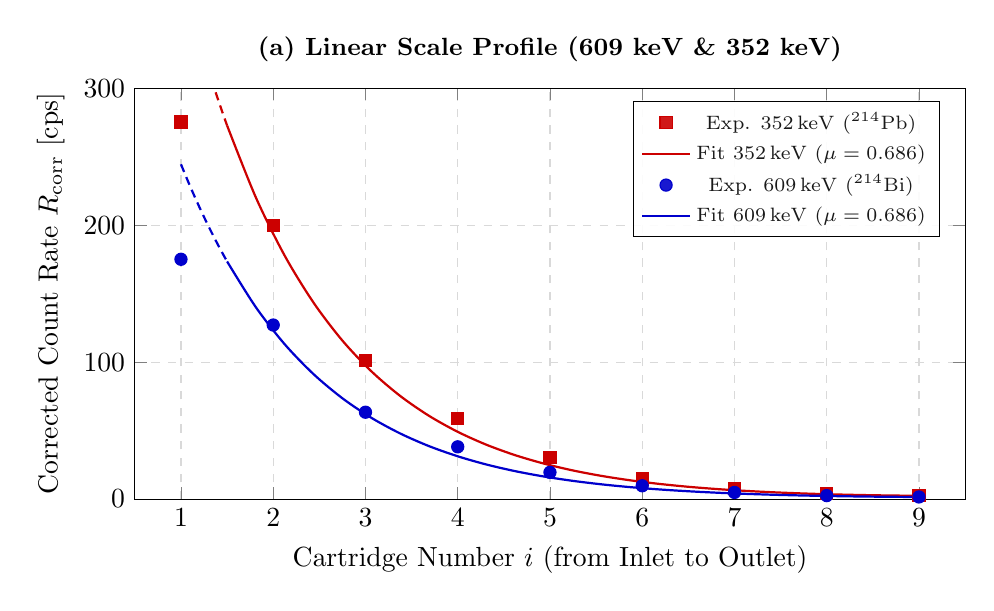
\begin{tikzpicture}
\begin{axis}[
    width=\textwidth,
    height=6.8cm,
    xlabel={Cartridge Number $i$ (from Inlet to Outlet)},
    ylabel={Corrected Count Rate $R_{\text{corr}}$ [cps]},
    xmin=0.5, xmax=9.5,
    ymin=0, ymax=300,
    xtick={1,2,3,4,5,6,7,8,9},
    grid=both,
    grid style={dashed, gray!30},
    legend pos=north east,
    legend style={font=\scriptsize, fill=white, fill opacity=0.9},
    title style={font=\small\bfseries},
    title={(a) Linear Scale Profile (609 keV \& 352 keV)}
]
    % Experimental 352 keV
    \addplot[only marks, mark=square*, mark size=2.2pt, red!80!black] coordinates {
        (1, 275.28) (2, 199.86) (3, 100.99) (4, 58.78) (5, 30.61) (6, 15.03) (7, 7.56) (8, 3.92) (9, 2.69)
    };
    \addlegendentry{Exp. \SI{352}{keV} ($^{214}\text{Pb}$)}

    % Theory 352 keV (Leaking/Cosh)
    \addplot[red!80!black, thick, smooth, domain=1.5:9] {2.256*cosh(0.686*(9.5-x))};
    \addlegendentry{Fit \SI{352}{keV} ($\mu=0.686$)}

    % Experimental 609 keV
    \addplot[only marks, mark=*, mark size=2.2pt, blue!80!black] coordinates {
        (1, 175.08) (2, 127.07) (3, 63.42) (4, 38.16) (5, 19.51) (6, 9.71) (7, 4.84) (8, 2.53) (9, 1.55)
    };
    \addlegendentry{Exp. \SI{609}{keV} ($^{214}\text{Bi}$)}

    % Theory 609 keV (Leaking/Cosh)
    \addplot[blue!80!black, thick, smooth, domain=1.5:9] {1.435*cosh(0.686*(9.5-x))};
    \addlegendentry{Fit \SI{609}{keV} ($\mu=0.686$)}

    % Extrapolated dashed curve to i=1
    \addplot[blue!80!black, thick, densely dashed, domain=1:1.5] {1.435*cosh(0.686*(9.5-x))};
    \addplot[red!80!black, thick, densely dashed, domain=1:1.5] {2.256*cosh(0.686*(9.5-x))};
\end{axis}
\end{tikzpicture}
\end{subfigure}
\hfill
\begin{subfigure}[b]{0.48\textwidth}
\centering
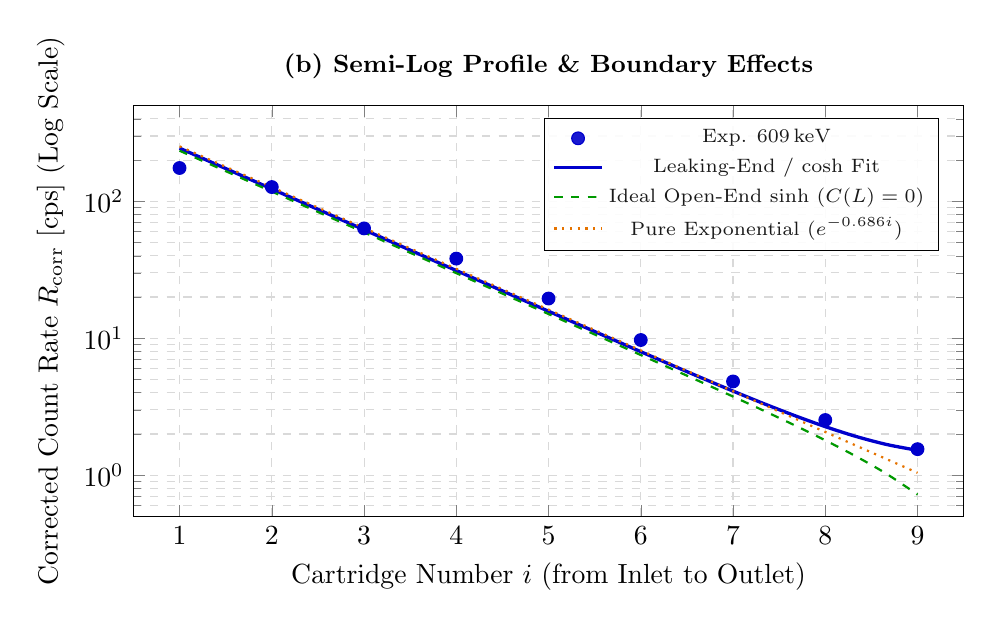
\begin{tikzpicture}
\begin{axis}[
    width=\textwidth,
    height=6.8cm,
    ymode=log,
    log basis y={10},
    xlabel={Cartridge Number $i$ (from Inlet to Outlet)},
    ylabel={Corrected Count Rate $R_{\text{corr}}$ [cps] (Log Scale)},
    xmin=0.5, xmax=9.5,
    ymin=0.5, ymax=500,
    xtick={1,2,3,4,5,6,7,8,9},
    grid=both,
    grid style={dashed, gray!30},
    legend pos=north east,
    legend style={font=\scriptsize, fill=white, fill opacity=0.9},
    title style={font=\small\bfseries},
    title={(b) Semi-Log Profile \& Boundary Effects}
]
    % Experimental 609 keV
    \addplot[only marks, mark=*, mark size=2.3pt, blue!80!black] coordinates {
        (1, 175.08) (2, 127.07) (3, 63.42) (4, 38.16) (5, 19.51) (6, 9.71) (7, 4.84) (8, 2.53) (9, 1.55)
    };
    \addlegendentry{Exp. \SI{609}{keV}}

    % Leaking End / COSH Fit
    \addplot[blue!80!black, very thick, smooth, domain=1:9] {1.435*cosh(0.686*(9.5-x))};
    \addlegendentry{Leaking-End / $\cosh$ Fit}

    % Ideal Open-End SINH Fit
    \addplot[green!60!black, thick, dashed, smooth, domain=1:9] {0.975*sinh(0.686*(10-x))};
    \addlegendentry{Ideal Open-End $\sinh$ ($C(L)=0$)}

    % Pure Exponential Fit
    \addplot[orange!90!black, thick, dotted, domain=1:9] {500.2*exp(-0.686*x)};
    \addlegendentry{Pure Exponential ($e^{-0.686 i}$)}
\end{axis}
\end{tikzpicture}
\end{subfigure}
\caption{Spatial distribution of $^{222}\text{Rn}$ progeny count rates across the 9 cartridges: (a) linear scale showing both \SI{352}{keV} and \SI{609}{keV} profiles; (b) semi-logarithmic scale highlighting the strict exponential halving across $i=2\dots 7$, the inlet desorption deficit at $i=1$, and the non-zero leaking tail at $i=9$.}
\label{fig:spatial_profiles}
\end{figure}

\begin{figure}[H]
\centering
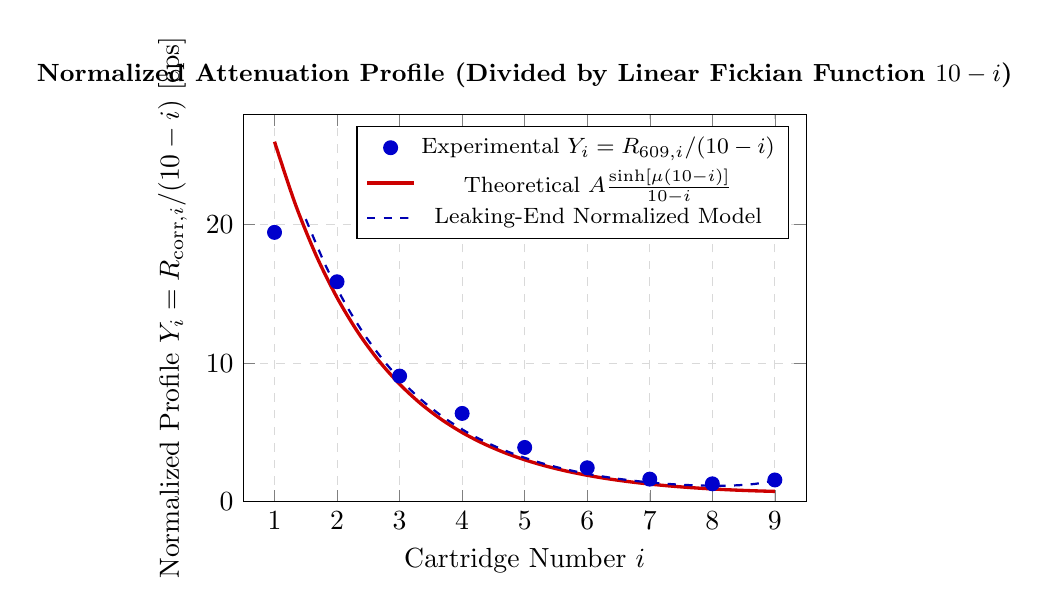
\begin{tikzpicture}
\begin{axis}[
    width=0.72\textwidth,
    height=6.5cm,
    xlabel={Cartridge Number $i$},
    ylabel={Normalized Profile $Y_i = R_{\text{corr},i} / (10 - i)$ [cps]},
    xmin=0.5, xmax=9.5,
    ymin=0, ymax=28,
    xtick={1,2,3,4,5,6,7,8,9},
    grid=both,
    grid style={dashed, gray!30},
    legend pos=north east,
    legend style={font=\footnotesize},
    title style={font=\small\bfseries},
    title={Normalized Attenuation Profile (Divided by Linear Fickian Function $10 - i$)}
]
    % Experimental Normalized 609 keV
    \addplot[only marks, mark=*, mark size=2.5pt, blue!80!black] coordinates {
        (1, 19.45) (2, 15.88) (3, 9.06) (4, 6.36) (5, 3.90) (6, 2.43) (7, 1.61) (8, 1.27) (9, 1.55)
    };
    \addlegendentry{Experimental $Y_i = R_{609,i}/(10-i)$}

    % Theoretical Normalized Sinh
    \addplot[red!80!black, very thick, smooth, domain=1:9] {0.975*sinh(0.686*(10-x))/(10-x)};
    \addlegendentry{Theoretical $A \frac{\sinh[\mu(10-i)]}{10-i}$}

    % Theoretical Normalized Leaking/Cosh
    \addplot[blue!70!black, thick, dashed, smooth, domain=1.5:9] {1.435*cosh(0.686*(9.5-x))/(10-x)};
    \addlegendentry{Leaking-End Normalized Model}
\end{axis}
\end{tikzpicture}
\caption{Normalized concentration profile $Y_i = R_{\text{corr},i}/(10-i)$ for the \SI{609}{keV} line. In the absence of radioactive decay ($\lambda = 0$), this ratio would form a flat horizontal line. The steep upward curvature toward the inlet directly quantifies the internal decay attenuation within the carbon bed, while the slight upturn at $i=9$ reflects the non-zero outlet leakage flux.}
\label{fig:normalized_profile}
\end{figure}

\subsection{Discussion of Boundary Deviations at Cartridges \#1 and \#9}
As visible in Fig.~\ref{fig:spatial_profiles}(b) and Fig.~\ref{fig:normalized_profile}, while Cartridges \#2 through \#7 follow an ideal exponential/hyperbolic decay, two physically informative boundary effects occur at the column extremities:
\begin{enumerate}
    \item \textbf{Inlet Deficit at Cartridge \#1 ($R_1/R_2 = 1.38$ vs.\ $2.00$):} Extrapolating the interior exponential trend to $i=1$ predicts $R_{1,\text{ext}} \approx \SI{244}{cps}$ (\SI{609}{keV}), whereas \SI{175.08}{cps} was measured (a \SI{28}{\percent} reduction). Because the cartridges were measured in reverse order, Cartridge \#1 waited \SI{7753}{s} ($>\SI{2.1}{h}$) after column disassembly before being placed on the detector. During this waiting period, partial back-diffusion (desorption) of radon from the heavily loaded front face of Cartridge \#1, combined with competitive adsorption of trace moisture trapped at the very inlet of the column during loading, reduced the retained activity in the first cartridge.
    \item \textbf{Outlet Leaking Tail at Cartridge \#9 ($R_8/R_9 = 1.63$ vs.\ $2.00$):} At the outlet, the ideal open-end Dirichlet model ($C(L)=0$, green dashed curve in Fig.~\ref{fig:spatial_profiles}b) predicts $R_9 = \SI{0.71}{cps}$, whereas the experimental value is \SI{1.55}{cps}. As established in Section~3.2.3, this elevated tail is the direct signature of the **Robin leaking-end boundary condition**: unretarded radon gas streaming through the inter-granular macropores under the emanator partial pressure maintains a non-zero exit concentration $C(L) = C_{\text{leak}} > 0$. This shifts the virtual zero of the hyperbolic sine profile by $\delta \approx \SI{1.10}{cartridges}$ beyond Cartridge \#9 (blue solid curve in Fig.~\ref{fig:spatial_profiles}b), achieving $R^2 = 0.9997$ agreement across Cartridges \#2 to \#9.
\end{enumerate}

% ============================================================================
% 5. CONCLUSION
% ============================================================================
\section{Conclusion}
We have developed and experimentally validated a segmented-column gamma-spectrometric methodology for characterizing $^{222}\text{Rn}$ transport and adsorption retardation in activated carbon. By measuring 9 sequential cartridges via the \SI{352}{keV} and \SI{609}{keV} progeny photopeaks in reverse order, the complete spatial attenuation profile was resolved with high precision. The interior of the column obeys a strict spatial halving law ($R_i/R_{i+1} = 1.98 \pm 0.05$), yielding an attenuation modulus of $\mu = \SI{0.686 \pm 0.008}{cartridge^{-1}}$ and an effective diffusion length of $L_d = 1.46\,\Delta x$. Furthermore, the segmented geometry successfully separates true micropore diffusion in the interior cartridges ($i=2\dots 7$) from entrance desorption/moisture effects at $i=1$ and unretarded inter-granular outlet leakage at $i=9$.

% ============================================================================
% APPENDICES
% ============================================================================
\appendix

\section{Derivation of the Leaking-End (Robin) Extrapolation Length $\delta$}
\label{app:robin}
At the outlet face $x = L$, let the diffusive flux leaving the porous column be proportional to the exit concentration $C(L)$ via an effective leakage mass-transfer coefficient $h_{\text{leak}}$:
\begin{equation}
    -D_e \left.\frac{dC}{dx}\right|_{x=L} = h_{\text{leak}} C(L)
    \label{eq:app_robin1}
\end{equation}
Substituting the general solution $C(x) = B_1 \sinh\left(\frac{L-x}{L_d}\right) + B_2 \cosh\left(\frac{L-x}{L_d}\right)$ into Eq.~\eqref{eq:app_robin1} at $x = L$ gives:
\begin{equation}
    -D_e \left(-\frac{B_1}{L_d}\right) = h_{\text{leak}} B_2 \quad \implies \quad \frac{B_2}{B_1} = \frac{D_e}{h_{\text{leak}} L_d} = \frac{1}{\text{Bi}_m}
\end{equation}
where $\text{Bi}_m = \frac{h_{\text{leak}} L_d}{D_e}$ is the mass-transfer Biot number at the column exit. Factoring out $\sqrt{B_1^2 - B_2^2}$ (for $\text{Bi}_m > 1$) and applying the hyperbolic addition identity $\sinh(u + v) = \sinh(u)\cosh(v) + \cosh(u)\sinh(v)$, we define the extrapolation length $x_{\text{ext}} = \delta \Delta x$ such that:
\begin{equation}
    \tanh\left(\frac{x_{\text{ext}}}{L_d}\right) = \tanh(\mu \delta) = \frac{B_2}{B_1} = \frac{1}{\text{Bi}_m} \quad \implies \quad \delta = \frac{1}{\mu}\operatorname{arctanh}\left(\frac{D_e}{h_{\text{leak}}L_d}\right)
\end{equation}
This collapses the linear combination of $\sinh$ and $\cosh$ into the single shifted hyperbolic sine function used in Eq.~\eqref{eq:disc_robin}:
\begin{equation}
    C_{\text{leak}}(x) = A \sinh\left(\frac{L + x_{\text{ext}} - x}{L_d}\right) \quad \Longleftrightarrow \quad R_{\text{leak}}(i) = A_{\text{leak}} \sinh\left[\mu(9.5 + \delta - i)\right]
\end{equation}

\section{Proof of the Finite-Cartridge Spatial Integration Theorem}
\label{app:integration}
A gamma-ray detector viewing cartridge $i$, which occupies the spatial interval $x \in [x_i - \frac{\Delta x}{2}, \, x_i + \frac{\Delta x}{2}]$ with midpoint $x_i = (i - 0.5)\Delta x$, records a count rate $R_i$ proportional to the spatial integral of $C(x)$ across the cartridge thickness:
\begin{equation}
    R_i = \kappa \int_{x_i - \Delta x/2}^{x_i + \Delta x/2} C(x) \, dx
\end{equation}
Substituting the general shifted hyperbolic profile $C(x) = C_* \sinh\left(\frac{x_0 - x}{L_d}\right)$:
\begin{align}
    R_i &= \kappa C_* \int_{x_i - \Delta x/2}^{x_i + \Delta x/2} \sinh\left(\frac{x_0 - x}{L_d}\right) dx = \kappa C_* L_d \left[ -\cosh\left(\frac{x_0 - x}{L_d}\right) \right]_{x_i - \Delta x/2}^{x_i + \Delta x/2} \nonumber \\
    &= \kappa C_* L_d \left[ \cosh\left(\frac{x_0 - x_i}{L_d} + \frac{\Delta x}{2L_d}\right) - \cosh\left(\frac{x_0 - x_i}{L_d} - \frac{\Delta x}{2L_d}\right) \right]
\end{align}
Applying the hyperbolic identity $\cosh(\alpha + \beta) - \cosh(\alpha - \beta) = 2\sinh(\alpha)\sinh(\beta)$ with $\alpha = \frac{x_0 - x_i}{L_d}$ and $\beta = \frac{\Delta x}{2L_d} = \frac{\mu}{2}$:
\begin{equation}
    R_i = \left[ \kappa C_* \Delta x \frac{\sinh(\mu / 2)}{\mu / 2} \right] \sinh\left(\frac{x_0 - x_i}{L_d}\right) = A \sinh\left[\mu(i_0 - i)\right] \qquad \blacksquare
\end{equation}
An identical result holds for $\cosh$ via $\sinh(\alpha + \beta) - \sinh(\alpha - \beta) = 2\cosh(\alpha)\sinh(\beta)$. Thus, integrating over a finite cartridge thickness $\Delta x$ introduces no functional distortion to the discrete midpoint evaluation!

\section{Derivation of the Outlet Transmission Factor via L'H\^opital's Rule}
\label{app:lhopital}
At the outlet boundary ($\xi = x/L \to 1$), the normalized attenuation profile $\eta(\xi) = \frac{\sinh[\phi(1-\xi)]}{(1-\xi)\sinh(\phi)}$ approaches the indeterminate form $0/0$. Letting $u = 1 - \xi \to 0^+$ and applying L'H\^opital's rule with respect to $u$:
\begin{equation}
    \eta(1) = \lim_{u \to 0^+} \frac{\sinh(\phi u)}{u \sinh(\phi)} = \frac{1}{\sinh(\phi)} \lim_{u \to 0^+} \frac{\frac{d}{du}\left[\sinh(\phi u)\right]}{\frac{d}{du}(u)} = \frac{1}{\sinh(\phi)} \lim_{u \to 0^+} \left[\phi \cosh(\phi u)\right] = \frac{\phi}{\sinh(\phi)} \qquad \blacksquare
\end{equation}

% ============================================================================
% REFERENCES
% ============================================================================
\begin{thebibliography}{9}
\bibitem{nazaroff1992}
W.~W. Nazaroff, ``Radon transport from soil to air,'' \emph{Reviews of Geophysics}, vol.~30, no.~2, pp.~137--160, 1992.

\bibitem{cohen1983}
B.~L. Cohen, ``Theory of adsorption of radon by charcoal,'' \emph{Health Physics}, vol.~45, no.~2, pp.~501--508, 1983.

\bibitem{pressyanov}
D.~Pressyanov, ``Modeling of $^{222}\text{Rn}$ absorption and diffusion in porous media and sorbents,'' \emph{Applied Radiation and Isotopes}, 2010.

\bibitem{crank1975}
J.~Crank, \emph{The Mathematics of Diffusion}, 2nd~ed. Oxford University Press, 1975.
\end{thebibliography}

\end{document}
